\chapter{Introduction}
\section{Background}
It is little or no alternative for the vast majority of trade over the world to transport by ship, in which case ship routing is a significant task during the voyage. With this task, ship could follow a safe and efficient path which is helpful for improving delivery efficiency and shortening delivery time. So, efficient ship routing is meaningful for both shipping itself and the entire industry chain.
\\However, in recent years, it is very hard to keep improving the performance of ship engines. Instead, finding an efficient path would play a more important role in reducing fuel consumption. Moreover, the concept of the `green shipping' has been raised in the international shipping industry and whithin the foreseeable future, shipping will still be dependent on fossil fuels. Therefore, an optimum path means not only economic efficiency but also environment protection to prevent pollution.
\begin{figure}[H]  
	\centering  
	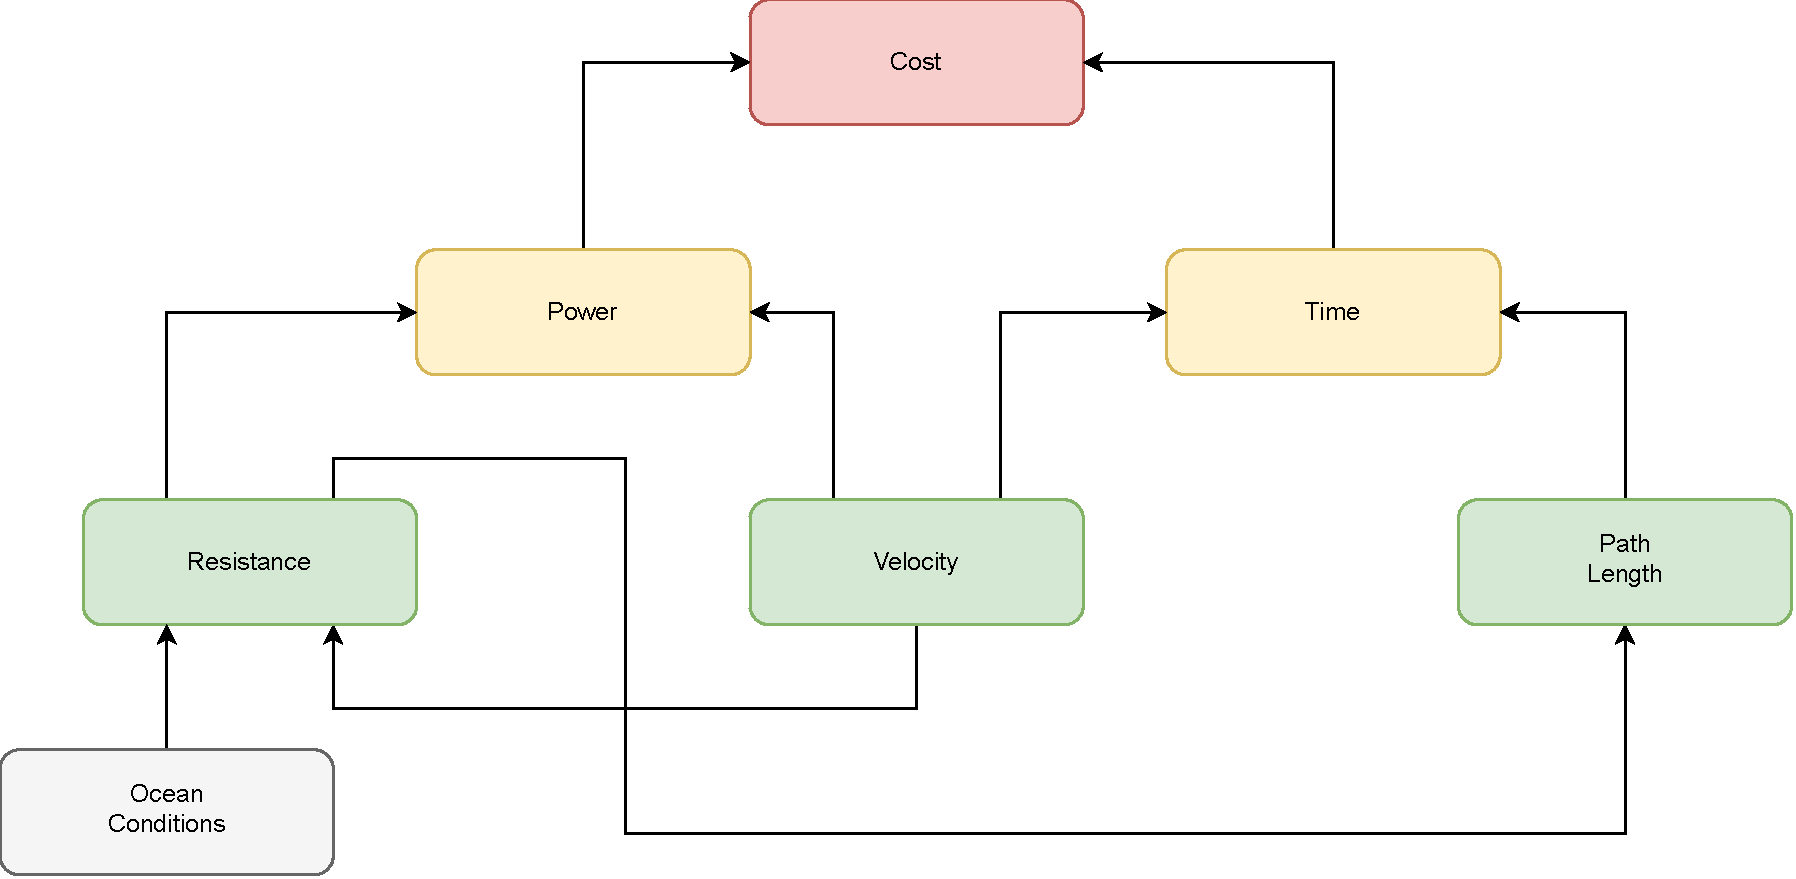
\includegraphics[width=0.9\linewidth]{cost function.pdf}  
	\caption{Cost analysis}  
	\label{CostFunc}  
\end{figure}
\noindent For a single voyage, the trip cost and its causes need to be discussed. Usually, this cost would be defined as the fuel consumption or the needed energy in this voyage, and it would be affected by two parameters, power per moment and task time. To calculate power, we need know the velocity and resistance of each moment. On the other side, the ship resistance would be affected by the velocity as well. Apart from ship velocity, the ocean environment is the other reason we need to take into account in resistance calculation, because these conditions would change if the ship follow different paths. Other elements, like ship parameters, are also important for resistance, but in this case, we could do nothing on these elements. The time to complete the task depends on the velocity of ship and the length of chosen path. To choose this path, the resistance is almost the most significant basis. In conclusion, as shown in \autoref{CostFunc}, environment conditions, ship velocities, resistance and path length must be discussed to find an efficient path.

\section{Objective}
In this project, a ship needs to transport load from point A to point B within a given time, in which case the optimal route, with respect to fuel consumption given some weather data, need to be shown. For this aim, costs of different places under different velocities and different heading angles would be calculated by various methods, like Hollenbach method, STAwave-1 method and ITTC method. Then, based on these data, total costs of different path would be calculated and compared by Dijkstra method. Then for each velocity, there would be one most efficient path, which could be compared again to find the optimal velocity causing minimum cost. To sum up, after several comparisons, the optimal route, the efficient velocity and the minimum cost would be found.

\section{Structure of the report}
Chapter 2 would tell more details about different methods used in this project.
\\Chapter 3 would introduce the programming tool and process, which would illustrate some important assumptions and the function of different codes.
\\Chapter 4 would contain some tests and discussion.
\\Chapter 5 would provide conclusion and recommendations for further work.